\documentclass[twocolumn,prl]{revtex4-1}
% \documentclass{article}
\usepackage{amsmath}
\usepackage{graphicx}
\usepackage{stfloats}

\begin{document}
\title{Capillary Forces Between Corners}
\author{Student A}
\author{Student B}
\author{Student C}
\author{Professor}
\affiliation{Brown University}

\begin{abstract}
% \lipsum
	Lorem ipsum dolor sit amet, consectetur adipisicing elit, sed do eiusmod tempor incididunt ut labore et dolore magna aliqua. Ut enim ad minim veniam, quis nostrud exercitation ullamco laboris nisi ut aliquip ex ea commodo consequat. Duis aute irure dolor in reprehenderit in voluptate velit esse cillum dolore eu fugiat nulla pariatur. Excepteur sint occaecat cupidatat non proident, sunt in culpa qui officia deserunt mollit anim id est laborum.
\end{abstract}

\maketitle

	Nearby interfacial objects mutually attract through capillary interactions in a shape-dependent mechanism commonly known as the Cheerios effect. It is a gravity and surface-wetting driven process that has been observed or postulated in dispersal of aquatic plant seeds\cite{peruzzo2013capillary}, directed colloidal self-assembly\cite{fan2004assembly} and locomotion of meniscus-climbing insects\cite{hu2005meniscus}. Thus far, focus has been primarily on objects initially far away or on a curved interface, cases where the interfacial deformation can be approximated by superposition of contributions from each individual objects. More recent studies elucidated the role of shape on the attraction between nearby objects using multipole expansions, and, in particular, on attraction near a sharp corner where there is a curvature singularity//cite//. Figure 1 presents qualitative observations of the attraction between two floating 1'' wide acrylic triangles as they approach each other, viewed from above. For a large class of relative initial positions and orientations, they rotate such that corners kiss first, after which they will fold or slide into a more stable final configuration. Prior to kissing, it appears that attraction is localized to the corners due to the curvature singularity. To the best of our knowledge, the force of attraction due to corners have never been quantified before. In this letter, we show that it scales as a power law of distance. For the 60 $^{\circ}$ corners in Figure 1, the force of attraction scales as $d^{14/5}$, where $d$ is the distance between corners.

Consider two identical corners tethered in place with separation $d$ defined as the distance between the tips of each corner as is schematically shown in //fig//. Pinning the contact line to the corners forms the boundary conditions of the deformed interface. It is a free surface which satisfies the Young-Laplace equation
\begin{equation}
\bigtriangledown^2 u = \frac{u}{l_c^2}
\end{equation}
where u is the displacement from an initially flat surface, $l_c = \sqrt{\sigma\rho g}$ the capillary length, $\sigma$ the surface tension and $\rho$g the specific weight. 


























//Show experimental set-up//
\begin{figure*}[htb!]

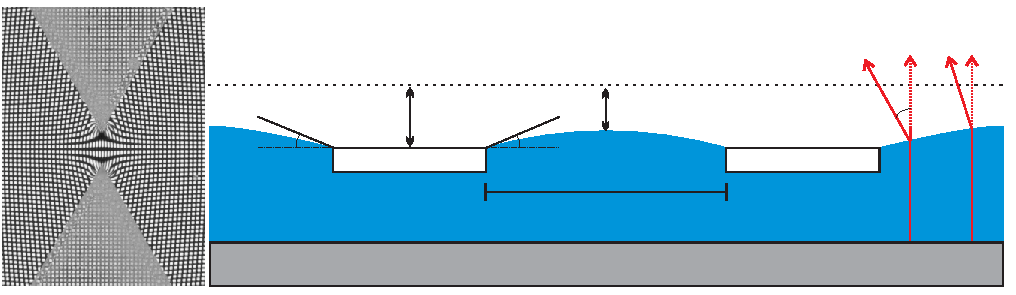
\includegraphics{Figures/Fig2.pdf}
\caption{Lorem ipsum dolor sit amet, consectetur adipisicing elit, sed do eiusmod tempor incididunt ut labore et dolore magna aliqua. Ut enim ad minim veniam, quis nostrud exercitation ullamco laboris nisi ut aliquip ex ea commodo consequat.}
\end{figure*}


\begin{equation}\label{eqn:forcebalance}
F \approx \frac{\sigma}{2} \int _C [(\frac{u^2}{l_c^2}- u_n^2 +u_t^2 )d\textbf{t} - 2u_n u_t d\textbf{n}]
\end{equation}
	the attractive force, $F$, by applying a force balance on a loop enclosing the meniscus\cite{he2013capillary}. u is the vertical displacement ... u/lc is the hydrostatic term and the gradients are the ...



//As a check, show attractive force between spheres and compare with literature//

Force from deformation of meniscus. Measure Meniscus deformations - Verify using circles. Use for triangles for d ~ lc and $d << lc$.

\section{Results}
//Show derivation for conformal mapping on angles//

//Show ux scaling for the inner and outer region//

//Show Force plot and regions of scaling//

\section{Discussion}
What does this mean?

Force concentrated at vertices is much stronger than force between smooth edges.

\section{Figures}
Figure 1: Analog of introduction in figures

Figure 2: Schematic for experiment and representative results 

Figure 3: Power law scaling and force vs. distances.

Figure 4: On the boundary integral methods

\section{notes}


\bibliographystyle{plain}
\bibliography{article}
\end{document}
